%*****************************************
\chapter{Tables}\label{ch05:tables}
%*****************************************

Excel workbooks are designed to store lots of information and organizing this information so that they display meaningful data can be challenging. Excel has many features that can help organize data and find needed information efficiently. Setting up data as a table from the onset will allows users to sort, filter, total, and subtotal the data easily. In Excel, a table is a collection of data about a particular subject stored in adjacent rows and columns. Tables can improve the look and feel of a workbook. This chapter explores how to best set up Excel tables, how to edit them, and then how to work with them effectively. These skills will be demonstrated in the context of a multi-sheet file that shows national average weather for two very different cities in the United States. Weather data is often voluminous and difficult to summarize since so much is collected every hour of every day and providing meaningful summaries of such data is a useful skill. The skills learned using weather data in this chapter can be be transferred to data found in any discipline or field.


\section{Table Basics}


Learning Objectives


1. Understand table structure.
2. Plan, create, and edit a table.
3. Freeze rows and columns.
4. Sort data in a table.




This section reviews the fundamental skills for setting up and maintaining an Excel table. The
objective used for this chapter is the construction of a multi-sheet file to keep track of two cities’
national weather data for the month of January. Organizing, maintaining, and reporting data are
essentials skills for employees in most industries.

Figure 5.1 shows the completed workbook that will be demonstrated in this chapter. Notice that
this workbook contains three worksheets. The first worksheet lists average weather for January in
Portland, Maine. The second sheet lists average weather data for January in a very different climate –
Portland, Oregon. The third sheet adds a weekly column to the Portland, Oregon data so that it can
be subtotaled by week.


\begin{figure}[H]
	\centering
	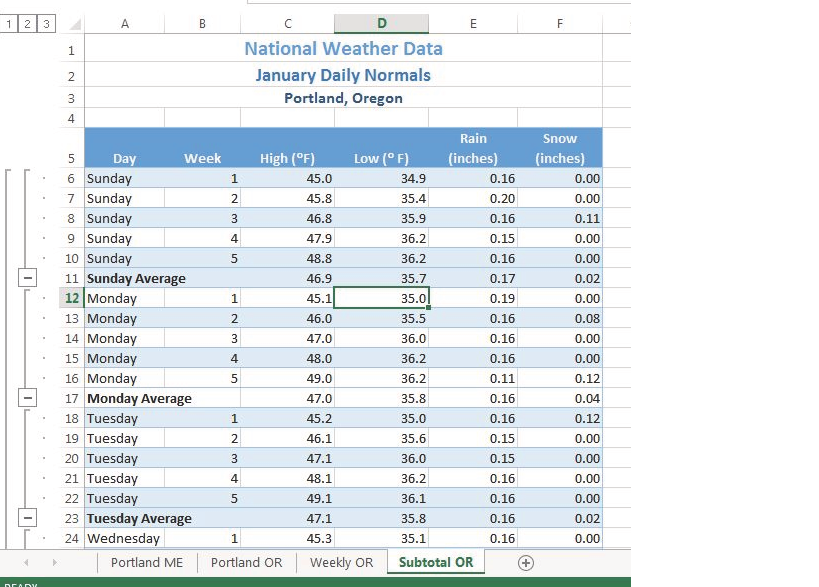
\includegraphics[width=\maxwidth{.95\linewidth}]{gfx/ch05_fig01}
	\caption{Completed National Weather Workbook}
	\label{05:fig01}
\end{figure}






\subsection{Creating a Table}

Download Data file: CH5 Data

When data is presented in long lists or columns, it helps if the table is set up well. Here are some rules
of data-entry etiquette to follow when creating a table from scratch:

1. Whenever you can, organize your information using adjacent (neighboring) columns and rows.
2. Start the table in the upper-left corner of the worksheet and work your way down the sheet.
3. Don’t skip columns and rows just to “space out” the information. (To place white space between
information in adjacent columns and rows, you can widen columns, heighten rows, and change
the alignment.)
4. Reserve a single column at the left edge of the table for the table’s row headings or identifying
information.
5. Reserve a single row at the top of the table for the table’s column headings.
6. If your table requires a title, put the title in the row(s) above the column headings.

Following these rules will help insure that the sorts, filters, totals, and subtotals you apply to your
table with give you the desired results.



With these rules in mind, we will begin working on the Portland ME worksheet in the National
Weather workbook. Notice that the data is in adjacent columns and rows. The upper-left corner of
the table is in A5 and the titles are above the column headings in Row 5. Since the set-up of our data
looks good, we are ready to turn our data range into an Excel table:

1. Open data file CH5 Data and save a file to your computer as CH5 National Weather.
2. Click on A5 in the Portland ME sheet.
3. Click the Table button in the Insert tab of the Ribbon.
Figure 5.2 will appear on your screen.


\begin{figure}[H]
	\centering
	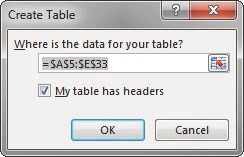
\includegraphics[width=\maxwidth{.95\linewidth}]{gfx/ch05_fig02}
	\caption{Create Table}
	\label{05:fig02}
\end{figure}





1. Make sure “My table has headers” is checked. Click OK.
2. Click in A5 again.
3. Adjust your columns widths so that you can see the complete headings in row 5 with the filter
arrows showing. The filter arrows are the down-arrow buttons that will appear in row 5 when
you create your table. We will learn how to use these to sort and filter later in this chapter.

After this, your spreadsheet will look like Figure 5.3.


\begin{figure}[H]
	\centering
	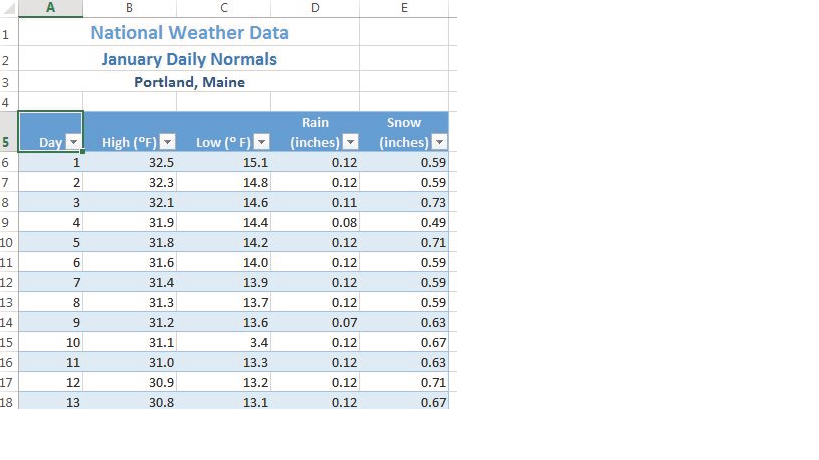
\includegraphics[width=\maxwidth{.95\linewidth}]{gfx/ch05_fig03}
	\caption{Weather Table}
	\label{05:fig03}
\end{figure}






Notice that a new ribbon tab, Table Tools Design, appears when you click inside your table. This
ribbon tab allows you to edit, style, and add functionality to your table.

Let’s try these steps again in the following steps:

1.    Click on the Portland OR sheet and click in cell A5.
2.    Click the Table button in the Insert tab of the Ribbon.
3.    Make sure “My table has headers” is checked. Click OK.
4.    Click in A5 again.
5.    Adjust your columns widths so that you can see the complete headings in row 5 with the filter
arrows showing.




Skill Refresher


Create a Table

1. Click on the top left cell in your data.
2. Click the Table button in the Insert tab of the Ribbon.
3. Make sure “My table has headers” is checked. Click OK.
4. Click on the top left cell again.
5. Adjust your columns widths so that you can see the complete headings with the filter arrows showing.



\subsection{Formatting Tables}

There are many ways to format an Excel table. There are preset colored Table Styles with Light,
Medium, and Dark colors. There are also a variety of Table Style Options listed in Table 5.1.

Table 5.1 Table Style Options

Table Style          Description
Header Row           Top row of the table that includes column headings
Total Row            Row added to the bottom that applies column summary calculations
First Column         Formatting added to the left-most column in the table
Last Column          Formatting added to the right-most column in the table
Banded Rows          Alternating rows of color added to make it easier to see rows of data
Alternating columns of color added to make it easier to see columns of
Banded Columns
data
Filter Button        Button that appear at the top of each column that lists options for sorting and filtering


We’ll add some formatting to both of our Portland weather tables in the following steps:

1. Click on the Portland ME sheet in your file.

2. In the Table Tools Design tab, in the Table Styles group, click the More button. (Note: figure ch05\_fig99 inserted here.)

A gallery of table styles will appear as in Figure 5.4.

\begin{figure}[H]
	\centering
	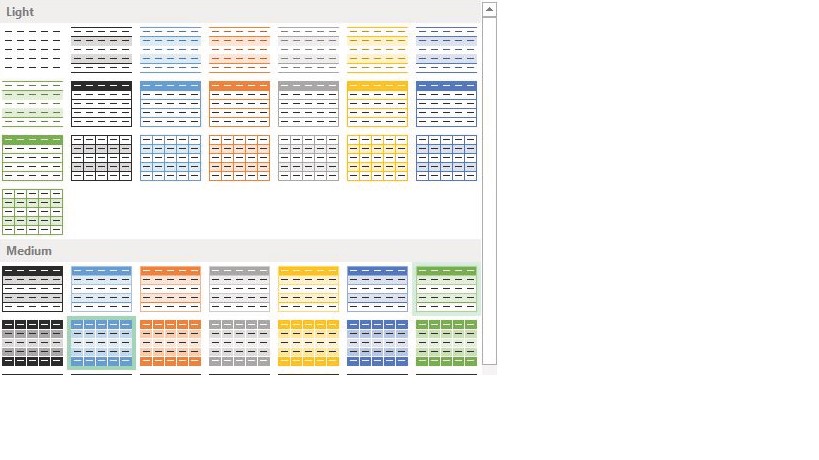
\includegraphics[width=\maxwidth{.95\linewidth}]{gfx/ch05_fig04}
	\caption{Table Styles}
	\label{05:fig04}
\end{figure}








3. In the Table Styles gallery, in the Medium Section, click Table Style Medium 7.

4. In the Table Style Options group in the Ribbon, click Banded Rows.

The alternating colored rows will disappear. The data in the table is now more difficult to read.

5. Try out some of the other options in the Table Style Options group. Once you’re finished, check
just Header Row, Banded Rows, and Filter Button as in Figure 5.5 below.


\begin{figure}[H]
	\centering
	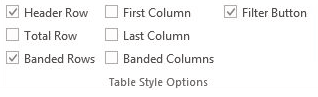
\includegraphics[width=\maxwidth{.95\linewidth}]{gfx/ch05_fig05}
	\caption{Ribbon Table Style Options}
	\label{05:fig05}
\end{figure}





\subsection{Adding Data to Tables}

Over time, you will need to add new data to an Excel table. You will add the data to the table in a blank
row. The easiest way to do this is to enter the data in the first blank row below the last row in the
table. You can then rearrange the data in the table by sorting it. If you need to add data in a specific
place in the middle of a table, you can insert a blank row in the middle and add your data there.

We need to add the last three days of the months to both our Portland, Maine and Portland, Oregon
tables. The following steps will walk you through doing this.

1. Click on the Portland ME worksheet.
2. Click on A34 (the left-most cell below the last row in the table).
3. Enter the following data:

Table 5.2 Portland, Maine data

Rain     Snow
Day High (°F) Low (°F)
(inches) (inches)
29    31.4       13.3       0.12       0.59
30    31.6       3.4        0.08       0.47
31    31.7       13.5       0.12       0.63




Notice that the banded row formatting continues as additional rows are added to the tables.

1. Click on the Portland OR worksheet.
2. Click on A34 (the left-most cell below the last row in the table).
3. Enter the following data:

Table 5.3 Portland, Oregon data



Rain     Snow
Day High (°F) Low (°F)
(inches) (inches)
29      48.8       36.2       0.16     0
30      49.0       36.2       0.11     0.32
31      49.1       36.1       0.16     0


\subsection{Finding and Editing Data}

It is inevitable that you will find data errors in your table and need to correct them. While you can
visually scan through a table to find your errors, this can be a tedious and tiresome process. Excel can
help with this through the Find command. When you use Find, the best practice is to start at the top
of the table to ensure that all your data is included in the search.

We know that a temperature of 3.4 degrees (brrr!) was entered erroneously in the Portland Maine
sheet. It should have been 13.4. To fix this error, complete the following steps.

1.    Click on the Portland ME sheet.
2.    Press the CTRL+HOME keys together to go to the top of the sheet (A1).
3.    In the Home tab of the ribbon, click on Find \& Select in the Editing Group and then click Find.
4.    In the Find box, type 3.4, and then click Find Next.


\begin{figure}[H]
	\centering
	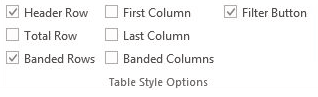
\includegraphics[width=\maxwidth{.95\linewidth}]{gfx/ch05_fig05}
	\caption{Find and Replace}
	\label{05:fig06}
\end{figure}





5. Click the Close button.
6. Replace 3.4 in the Low column for Day 10 with 13.4.
7. Now switch to the Portland Oregon sheet and find the Snow error of .32. Change it to 0.12. You
should find the error in Day 3.


Skill Refresher


Finding and Replacing Data

1. In the Home tab of the ribbon, click on Find \& Select in the Editing Group and then click Find.




2. In the Find box, type what you want to find, and then click Find Next.
3. Continuing click Find Next until you find.what you are looking for.
4. Click Close and edit your data.




\subsection{Freeze Rows and Columns}

When you freeze panes, Microsoft Excel keeps specific rows or columns visible in your table when
you scroll through it on your screen. For example, if the first row in your spreadsheet contains labels,
you might freeze that row to make sure that the column labels remain visible as you scroll down in
your spreadsheet. When we scroll through our weather data, it would be nice to keep our column
headings visible on the screen.

To freeze your headings:

1.   Click in A6, the left-most cell below the headings row.
2.   Click the View tab in the ribbon.
3.   Select Freeze Panes and then Freeze Panes again.
4.   Scroll up and down the sheet and notice that the headings are always displayed at the top of the
table.

\begin{figure}[H]
	\centering
	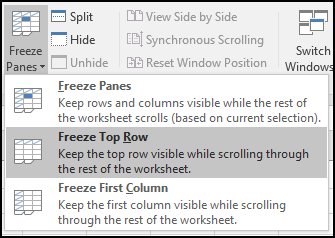
\includegraphics[width=\maxwidth{.95\linewidth}]{gfx/ch05_fig07}
	\caption{Freeze Pane}
	\label{05:fig07}
\end{figure}






To unfreeze your headings:

1. Click on the View tab in the ribbon.
2. Select Unfreeze Panes.

\subsection{Simple Sort}

Content in a table can be sorted alphabetically, numerically, and in many other ways. Sorting helps
organize data by one or more columns in your table. Table 5.4 describes the different sort orders
available for each column of data.

Table 5.4 Sort Options

Sort Order     Text                     Numbers               Dates
Smallest to Largest

Ascending      Alphabetical (A-Z)                             Chronological (oldest to newest)

Lowest to Highest
Largest to Smallest
Reverse Chronological (newest to
Descending Reverse Alphabetical (Z-A)
oldest)
Highest to Lowest


Let’s say we want to know what the snowiest day was in January in Portland, Maine; so we want to
sort the Snow column in Descending order so that the snowiest day ends up at the top of the table.

1. Click on the filter Click arrow to the right of the header Snow (inches) in the Portland ME
worksheet.
2. Click on the choice Click %ZA↓ Sort Largest to Smallest. See Figure 5.8 below.


\begin{figure}[H]
	\centering
	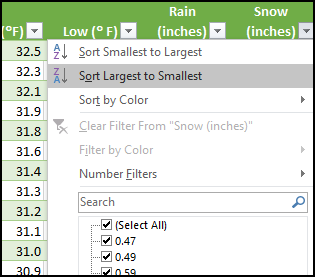
\includegraphics[width=\maxwidth{.95\linewidth}]{gfx/ch05_fig08}
	\caption{Sort by One Column}
	\label{05:fig08}
\end{figure}





If you did this correctly, you’ll see that the snowiest day at the top of the list in January 3rd (in row 6)
with 0.73 inches of snow! Notice the filter arrow changes in the snow column to a downward
pointing arrow to indicate you sorted that column in descending order (largest to smallest).


\begin{figure}[H]
	\centering
	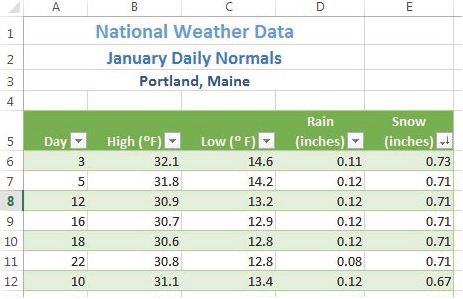
\includegraphics[width=\maxwidth{.95\linewidth}]{gfx/ch05_fig09}
	\caption{Snowiest Days in Maine}
	\label{05:fig09}
\end{figure}






3. Now switch to the Portland Oregon sheet and repeat these sort steps to find the snowiest day in
Oregon. Check your answers with Figure 5.10.

\begin{figure}[H]
	\centering
	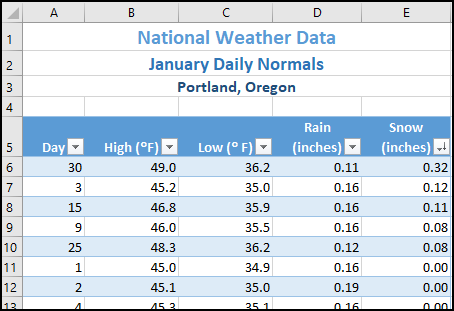
\includegraphics[width=\maxwidth{.95\linewidth}]{gfx/ch05_fig10}
	\caption{Snowiest Days in Oregon}
	\label{05:fig10}
\end{figure}






Skill Refresher


Sort a Column

1. Click on the filter Click arrow to the right of the header in the column you want to sort.
2. Click on the choice AZ! or %ZA↓ to sort your data by that column.




\subsection{Multi-Level Sort}

Sometimes you will need to sort your table by more than one column at a time in order to efficiently
analyze your data. For example, if you were looking at several different types of loans from several
bank offices, you would need to sort by the type of loan and then by bank office name to clearly see
the different groups of loans. If you had a list of grades for students over their time in high school,
you’d want to sort first by student name, but then also by grade level (freshman, sophomore, junior,
and senior) so that each student’s grades would appear in chronological order.

For our weather data, let’s look at the snow days in Oregon and see how cold they were!

1.   Click on the Portland OR sheet, then click on a cell in the table.
2.   Click on the Data tab in the ribbon and then click the Sort button.
3.   Click the down-arrow for Column and select Snow (inches).
4.   Click the down-arrow for Order and select Largest to Smallest.
5.   To add 2nd level sort, click on the Add Level button in the top left corner of the dialog box.
6.   In the new Then by row, click the down-arrow for Column and select Low (°F).
7.   In the same row, click the down-arrow for Order and select Smallest to Largest. Your dialog box
should look like Figure 5.11.

\begin{figure}[H]
	\centering
	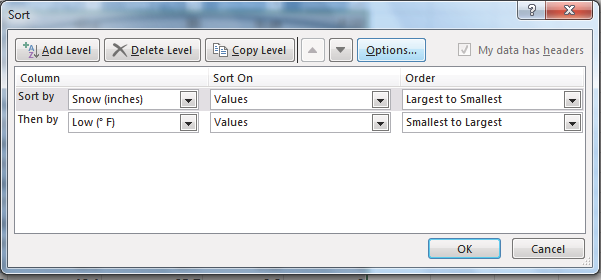
\includegraphics[width=\maxwidth{.95\linewidth}]{gfx/ch05_fig11}
	\caption{Multi-Level Sort}
	\label{05:fig11}
\end{figure}






8. Click OK. Your table sort results should look like Figure 5.12. Notice for the two days with 0.08
inches of snow, the low temp of 35.5 on Day 9 is displayed before the low temp of 36.2 on Day
25. The lowest of the two was listed first. Also notice that the filter arrows changed on the
sorted columns to show you how they are sorted.


\begin{figure}[H]
	\centering
	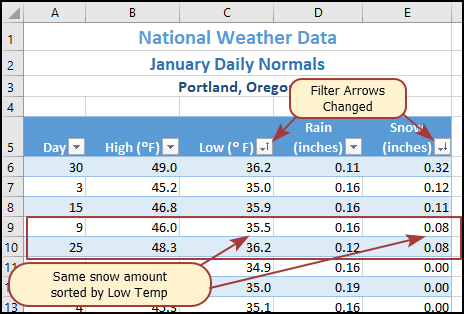
\includegraphics[width=\maxwidth{.95\linewidth}]{gfx/ch05_fig12}
	\caption{Multi-Level Sort Results}
	\label{05:fig12}
\end{figure}






\subsection{Custom Sorts}

In most cases, we want our data sorted in “typical” sort order: numbers sorted highest to lowest, words
sorted alphabetically, etc. Some data in our everyday lives; however, does not make sense when sorted
this way. For example, if you sorted the days of the week alphabetically, you’d get: Friday, Monday,
Saturday, Sunday, Thursday, Tuesday, and Wednesday. This order would be of no use to anyone!
Similarly, the months of the year would not make sense alphabetically. Can you think of a number
that would not make sense in either highest to lowest or lowest to highest order? (This is a good brain
teaser!)

In our weather data, we’ve added a column for the week in the Weekly OR sheet and changed the days
to Sunday through Saturday. This sheet lets us further analyze Portland, Oregon’s data to see if there
are weekly trends in the weather. Let’s see if we can sort the Weekly OR sheet by Week and then by
Day.

1.   Click on the Weekly OR worksheet.
2.   Click on A5 and insert a table.
3.   Click on Sort in the Data tab in the ribbon.
4.   Click the down-arrow for Column and select Week.
5.   Click the down-arrow for Order and select Smallest to Largest.
6.   To add 2nd level sort, click on the Add Level button in the top right corner of the dialog box.
7.   In the new Then by row, click the down-arrow for Column and select Day.
8.   Click the down-arrow for Order and select Custom List. The dialog box in Figure 5.13 will
appear on your screen.

\begin{figure}[H]
	\centering
	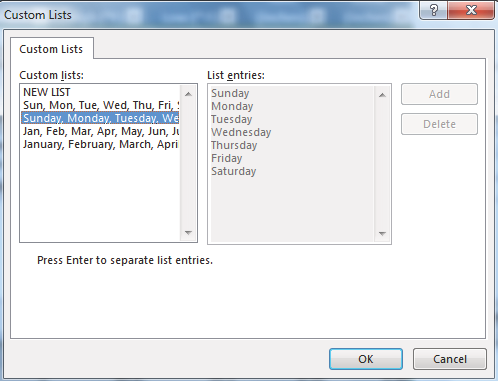
\includegraphics[width=\maxwidth{.95\linewidth}]{gfx/ch05_fig13}
	\caption{Custom Lists}
	\label{05:fig13}
\end{figure}







9. Click on Sunday, Monday, Tuesday, etc. in the Custom lists on the left-side of the dialog box.
NOTE: Make sure you select the days of the week spelled out, not the abbreviations for the days
of the week.
10. Click OK. Your Sort dialog box should look like Figure 5.14.


\begin{figure}[H]
	\centering
	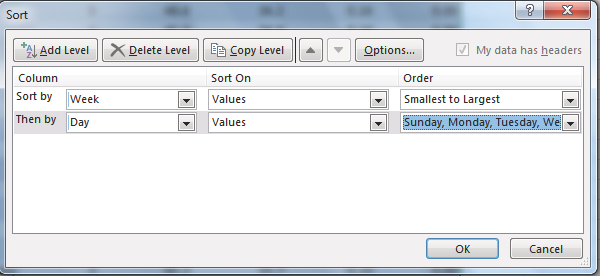
\includegraphics[width=\maxwidth{.95\linewidth}]{gfx/ch05_fig14}
	\caption{Sort Dialog Box}
	\label{05:fig14}
\end{figure}





11. Click OK again. Your sorted table should now look like Figure 5.15. Notice the data is in Week
order and, within each week, in Day order.
12. Save your work.


\begin{figure}[H]
	\centering
	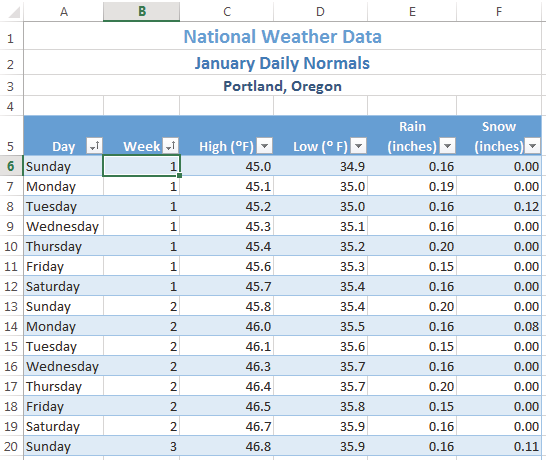
\includegraphics[width=\maxwidth{.95\linewidth}]{gfx/ch05_fig15}
	\caption{Custom Sort}
	\label{05:fig15}
\end{figure}








Key Takeaways


• Tables are made up of adjacent rows and columns of data with a single row of column headings at the top.

• You can create a table by clicking in the top left-most cell in your data and selecting Table in the Insert tab of
the ribbon.

• There are a gallery of styles, as well as, style options to choose from to format a table.

• When you need to add data, it is best to add it one row below the bottom of the table. You can then sort to
reorganize your data.

• Freezing heading keeps your column headings displayed while you scroll through your table data.

• You can use the filter arrows in the table headings to sort by a single column. Use Sort in the Data tab in the
ribbon to sort by two or more columns at a time.

• Custom Sorts can be used when data needs to be sorted in a special way (i.e. – Days of the Week).



\section{Intermediate Table Skills}




Learning Objectives


• Filter table data.

• Add a total row to a table.

• Insert subtotals into a table.



\subsection{Filtering Data}

When you first create an Excel table, filter arrows appear in all the column headings. We have seen
that you can use those arrows to sort your data by a single column. You can also use these same arrows
to filter or limit the data you see by narrowing the displayed data within a column. There are many
ways to filter data within a column depending on whether the data in the column is text or numeric.
Table 5.5 gives you some filter examples:

Table 5.5 Filter Examples

Text Filters
Desired Results                                     Filter Column Text Filter                         Checkbox Selected
Data for the State of New Jersey (NJ)               State            Equals NJ                        NJ
Data for Books that Have Gardening in Their Title Title              Contains Gardening
Data for Weather on the Weekend                     Day              Equals Saturday OR equals Sunday Saturday and Sunday




Numeric Filters
Desired Results                         Filter Column Number Filter                       Checkbox Selected
Data for Income Greater Than \$1,000 Income             Greater than 1,000
Data for Amount Paid Equal to Zero      Amount Paid    Equals 0.00                        0.00
Data for Mortgage and Auto Loans        Loan Type      Equals Mortgage OR equals Auto Mortgage and Auto


Notice there are sometimes more than one way to filter data (i.e. – with a filter choice or a checked
box). There are also single criteria filters, as well as, multi-criteria filters. We will explore all of these
next.

To start filtering, let’s look at just the first week of data in the Weekly OR sheet:

1.    Click on the Weekly OR sheet and click on a cell in the table.
2.    Click the filter arrow to the right of the Week heading.
3.    Click the Select All checkbox to deselect all of the checkbox choices.
4.    Click on 1 to select Week 1.
5.    Click OK.

Your table should look like Figure 5.16. You should see only 7 rows of Week 1 data in your table.
Notice in your Status Bar at the bottom of your screen the message “7 of 31 records found”. Also
notice that the filter arrow in the Week heading has changed to a funnel which indicates that this
column is currently filtered.


\begin{figure}[H]
	\centering
	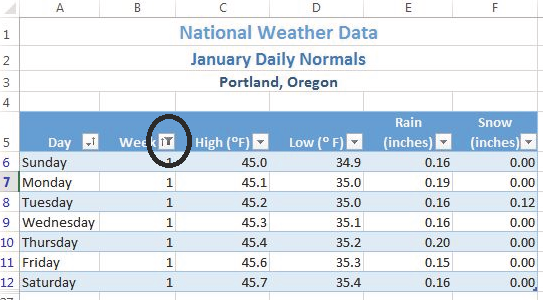
\includegraphics[width=\maxwidth{.95\linewidth}]{gfx/ch05_fig16}
	\caption{Filter}
	\label{05:fig16}
\end{figure}





To remove your filter:

1. Click the funnel next to the Week heading.
2. Select “Clear filter from Week”.


Skill Refresher


Filter a Column

1. Click the filter arrow to the right of the heading in the column you want to filter.
2. Click the Select All checkbox to deselect all of the checkbox choices.
3. Click on the checkboxes you want to filter by.
4. Click OK.

Un-Filter a Column

1. Click the funnel to the right of the heading in the column you filtered.
2. Select Clear filter.



Now let’s try a numeric filter. We want to find days in Portland ME when it’s warmer than 32
degrees in January:

1. Click in the Portland ME sheet, then click on a cell in the table.
2. Click on the filter arrow next to the High heading.
3. Click on Number filters, then select Greater than. The Custom AutoFilter dialog box will appear
on your screen.
4. Enter 32 in the space to the right of “is Greater than”. Your Custom AutoFilter dialog box should
now match Figure 5.17.


\begin{figure}[H]
	\centering
	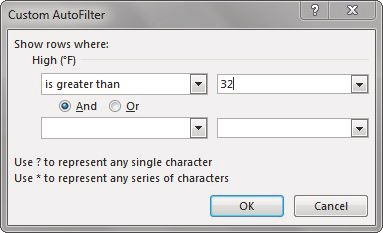
\includegraphics[width=\maxwidth{.95\linewidth}]{gfx/ch05_fig17}
	\caption{AutoFilter Dialog Box}
	\label{05:fig17}
\end{figure}





5. Click OK.

You should see that it was only above 32 degrees three days in January in Maine – the first
three! Check your table against Figure 5.18.


\begin{figure}[H]
	\centering
	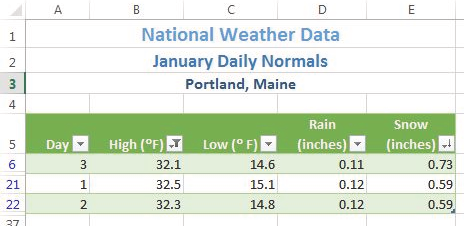
\includegraphics[width=\maxwidth{.95\linewidth}]{gfx/ch05_fig18}
	\caption{Maine Filter Results}
	\label{05:fig18}
\end{figure}




Let’s review sorting and filtering in the following steps:

1.   Click on the Weekly OR sheet and clear the Day column filter.
2.   Sort the table by Week (smallest to largest).
3.   Filter the table to only show Mondays.
4.   Compare your table results to Figure 5.19.

\begin{figure}[H]
	\centering
	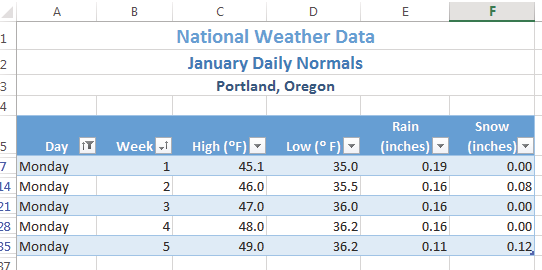
\includegraphics[width=\maxwidth{.95\linewidth}]{gfx/ch05_fig19}
	\caption{Oregon Filter Results}
	\label{05:fig19}
\end{figure}



\subsection{Filtering Using the Slicer}

Beginning in Excel 2013, slicers were added to the software as another way to filter your table data. A
slicer is really useful because it clearly indicates what data is shown in your table after you filter your
data.

Let’s try using the Slicer to filter our Portland OR data table:

1. Click on the Portland OR sheet and click in the table.
2. In the ribbon’s Table Tools Design tab, click Insert Slicer.
3. Click on Day in the Insert Slicers dialog box, and then click OK.
4. Drag the slicer so that the upper left-hand corner lines up with the top corner of cell G5.
5. Notice that when you insert a Slicer, a Slicer Options tab appears on the ribbon. This tab lets
you change the style and size of the entire slicer or the individual slicer buttons.
6. Click on the Slicer options tab, then click on the More button next to Slicer Styles. The choices
in Figure 5.20 will show on your screen.

\begin{figure}[H]
	\centering
	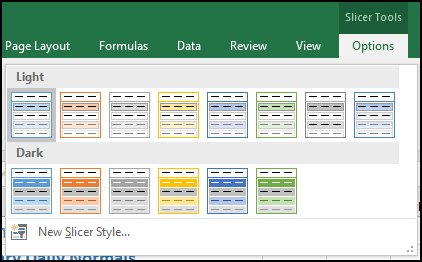
\includegraphics[width=\maxwidth{.95\linewidth}]{gfx/ch05_fig20}
	\caption{Slicer Styles}
	\label{05:fig20}
\end{figure}






1. Select the first choice under Dark.


2. In the Size group on the Slicer Options ribbon (NOT the Buttons group), change the width to 1”.
3. Click in the table and scroll down to Day 15 and click the 15 button to show only the data for
January 15th in the table.
4. Hold down the CTRL key and click on the Slicer buttons for Days 10 through 14. Your table
should now show the data from Days 10-15.
5. Sort the Day column in Ascending order to show the days in order as in Figure 5.21.


\begin{figure}[H]
	\centering
	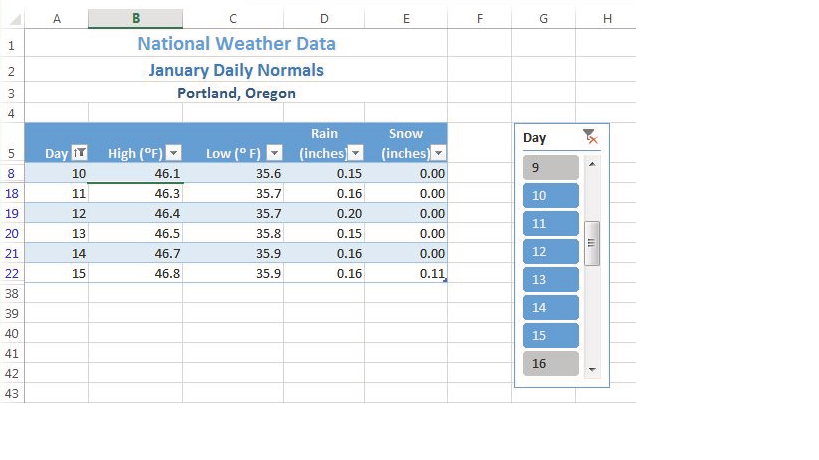
\includegraphics[width=\maxwidth{.95\linewidth}]{gfx/ch05_fig21}
	\caption{Slicer Results}
	\label{05:fig21}
\end{figure}





\subsection{Total Rows}

By adding a total row to the bottom of your table, you can quickly see summary data for one or more
of the columns in your table. Total rows can be added to tables as a whole, or those that are filtered.
Total rows can easily be toggled on and off as the need for summary data arises.

1. Click on the Portland ME sheet and clear the filter from the High column.
2. Click on the Total Row check box in the Table Style Options group in the Table Tools Design tab
in the ribbon.
3. Scroll to the bottom of your table to the Total Row. Notice the total for the Snow data.
4. Click on D37 (in the Rain column), and then click the down-arrow that appears to the right of
the cell.
5. Choose Sum to add a sum to the Total Row in the Rain column.
6. To see the Average rainfall for the month of January, click on the arrow again and choose
Average.
7. Repeat this step in E37 to see the Average snowfall.
8. Use the Decrease Decimal button in the Home tab of the ribbon to change the decimal places in
D37 and E37 to 2. Compare your Total Row to Figure 5.22.

\begin{figure}[H]
	\centering
	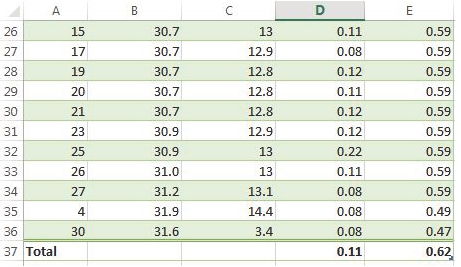
\includegraphics[width=\maxwidth{.95\linewidth}]{gfx/ch05_fig22}
	\caption{Total Row}
	\label{05:fig22}
\end{figure}





1. Now switch to the Weekly OR sheet and see if you can successfully add a Slicer and Total Row
to this table:
2. Clear the filter from the Day column.
3. Add a Slicer for the Day column to the sheet.
4. Move the top left corner of the slicer to H5. Resize it as needed and choose a Slicer Style.
5. Select Monday through Friday in the Slicer so that Saturday and Sunday data do NOT show in
your table.
6. Add a Total Row that averages the High and Low columns. Your averages should be High: 47.0
and Low: 35.8. Change the label “Total” to “Average” by clicking A37 and typing Average.


Skill Refresher


Add a Total Row

1. Click on the Total Row check box in the Table Style Options group in the Table Tools Design tab in the
ribbon.
2. Scroll to the bottom of your table to find the Total Row.
3. Click in one of the columns in the Total Row, and then click the down-arrow that appears to the right of
the cell.
4. Choose Sum to add a sum to the Total Row in the column.
5. To see the Average for column, click on the arrow again and choose Average.

Some other choices in the Total Row are Count (for words), Count Numbers, Max, and Min.




Skill Refresher


Add a Slicer



1. Click on Insert Slicer in the Table Tools Design tab in the ribbon.
2. Check the box for the column to which you want to add a Slicer.
3. Click OK.



\subsection{Subtotaling}

You can automatically calculate subtotals and grand totals in a table for a column. This is a powerful
tool that allows you to quickly display multiple levels of summary data within your table. This can
provide Management with a report of higher level summary data one minute, and then can be easily
switched back to detailed data the next minute. It is important to save often during this process and
follow the steps carefully. It is recommended that you make a copy of the data you want to subtotal
and place it in a new sheet, so that you can save the summary subtotaled data separately if desired.

In order to subtotal successfully, you always need to do the following in order:

1.   Sort by the column you want to subtotal on.
2.   Convert the table back to a normal Excel range. You cannot subtotal inside a table.
3.   Subtotal in the Data tab in the ribbon.
4.   If you want to limit your displayed data further, Filter in the Data tab in the ribbon.

We want to find out what the weather looks like for each day of the week, so we’ll need to save our
data to a new sheet, sort by the days of the week, and then convert the table in order to get ready to
see the subtotal.

1. Click on the Weekly OR sheet.
2. Point at the Weekly OR sheet tab at the bottom of the screen, hold the CTRL key down, and
left-drag the sheet to the right until you are past all the existing sheets.
3. When you see a sheet icon with a + sign, let go of the mouse button and then the CTRL key. A
Weekly OR (2) sheet will appear.
4. Right-click on the new Sheet tab, select Rename, type Subtotal OR, and then press ENTER.
5. Save your file before you start Subtotaling!
6. Remove all filters in the table by clicking the Data tab and then choosing Clear.
7. Now we want to Sort the table by the Day column using a Custom Sort in the Sort button in the
ribbon to sort in the order Sunday, Monday, Tuesday, etc. (See Figure 5.13 through 5.15 for a
review of Custom Sorting.)
8. Before you can subtotal, you must convert your table back to a regular range. To do this, click
Convert to Range in the Table Tools Design tab on the ribbon. (See Figure 5.23)


\begin{figure}[H]
	\centering
	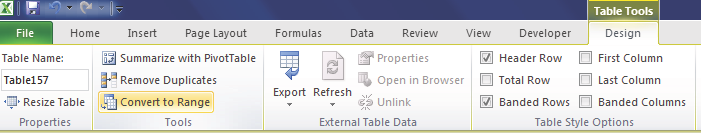
\includegraphics[width=\maxwidth{.95\linewidth}]{gfx/ch05_fig23}
	\caption{Convert to Range}
	\label{05:fig23}
\end{figure}





9. When asked if you want to convert the table, click Yes.
10. Because your data is no longer formatted as a table, your slicer will disappear; and you will no
longer have access to the Table Tools Design tab in the ribbon.
11. Under the Data tab in the ribbon, click Subtotal.
12. In the Subtotal Window, make the choices shown in the Figure 5.24. It is essential that you select
the column you sorted by in the “At each change in” field at the top of the window. Click OK.


\begin{figure}[H]
	\centering
	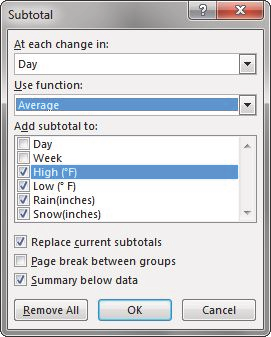
\includegraphics[width=\maxwidth{.95\linewidth}]{gfx/ch05_fig24}
	\caption{Subtotal Window}
	\label{05:fig24}
\end{figure}





Your data should look like Figure 5.25. Successful subtotaling shows only one subtotal for each group
in the column you sorted by. (HINT: If you end up with more than one Subtotal for the same group
(i.e – one of the days of the week in our example), you did not sort before subtotaling. Remove your
subtotals using the Remove All button in Figure 5.24, sort your table, and then try subtotaling again.)


\begin{figure}[H]
	\centering
	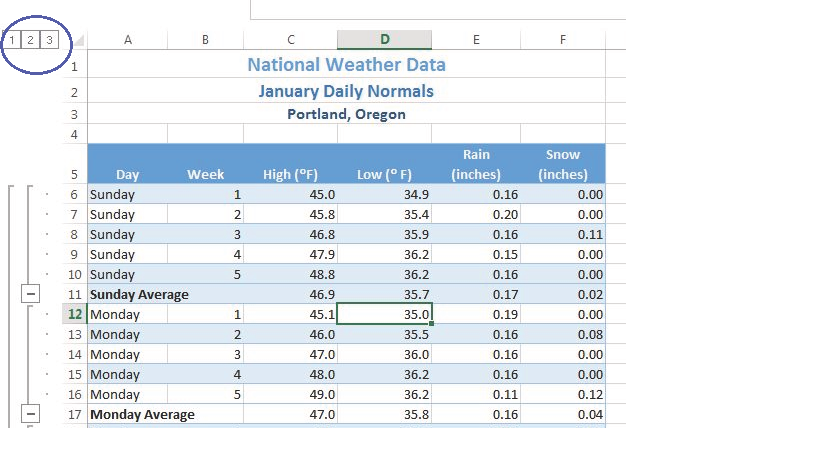
\includegraphics[width=\maxwidth{.95\linewidth}]{gfx/ch05_fig25}
	\caption{Subtotal Results}
	\label{05:fig25}
\end{figure}



Notice the three Outline buttons circled in the upper-left corner of the spreadsheet. These allow you
to control the amount of subtotaled data that is displayed. Table 5.5 describes the different Outline
buttons.

Table 5.5 Subtotal Outline Buttons

Button Content Displayed
Only grand total
Level 1


Subtotals and grand total
Level 2


Level 3 Individual records, subtotals, and grand total


Let’s try the three Outline buttons to see the difference in the data displayed:

1. Click on the 1 Outline button in the upper left-hand corner of the sheet.
2. You should see only the Grand Average row with averages for High, Low, Rain, and Snow.
3. Click on the 2 Outline button.
4. Now you’ll see the average for each day of the week along with the Grand Average.
5. Click on the + Sign button to the left of the Sunday Average row.
6. This expands just the Sunday Day data and displays the individual records for this subset of the
data. Clicking on + Sign buttons will expand a portion of the data at a time. Clicking on – Sign
buttons hide a portion of the data at a time.
7. Click on the 3 Outline button.

8. All the individual records along with the subtotals, and Grand Average should be displayed.
9. Save your Excel file.


Key Takeaways


• Filtering is an easy way to see a subset of your data. Filtering arrows appear to the right of each column
heading when you insert a table with a header row.

• You can filter by text or numerically.

• A slicer is another way to filter in Excel that provides a set of filtering buttons on your sheet.

• Adding a total row to a table is a quick, efficient way to see summary statistics for one or more columns in a
table.

• Subtotaling provides a way to quickly add totals to groups within a column along with providing a grand total
at the bottom of the table.

• Subtotal Outline buttons allow users to see add of the subtotaled data, just the totals and grand total, or
simply the grand total.

• Plus and minus buttons within subtotaling allow a user to expand and hide portions of the subtotaled data.



\section{Preparing to Print}




Learning Objectives


1. Review options for professional page setup for printing.
2. Understand how to insert a picture to enhance the visual appearance of a worksheet.
3. In this section, we will preview the worksheets containing tables to ensure they will print in a professional
manner. We will make any formatting and page setup changes that are needed, as well as add a picture to
one of the worksheets to enhance its appearance.



\subsection{Previewing a Worksheet}

Data file: Continue with CH5 National Weather

Now that the weather data has been sorted, filtered, and subtotaled as needed, it is time to print the
worksheets. You are going to start with the Portland ME worksheet.

1. Click on the Portland ME worksheet. If needed, use Ctrl-Home to move to cell A1.

Notice that cells A1, A2, and A3 are not merged and centered over the entire table of data. To fix this,
you need to unmerge each of the merged cells, and then merge them again, making sure to include E1,
E2, and E3 in the selection.

1. Select cell A1 and click the Merge \& Center button. This should split A1 into four cells (A1:D1).
2. Select the range A1:E1 and click the Merge \& Center button. Cell A1 should now be merged
across A1:E1.
3. Repeat steps 1 and 2 for A2 and A3.

Next you need to preview the worksheet in Print Preview and determine what page setup options
need to be set.

1. Go to Backstage view and select Print from the menu.

Notice that the table is to the far left of the page, with quite a bit of white space on the left. You decide
that it would look better centered on the page.




1. In the Settings section, click the link for Page Setup. This opens the Page Setup dialog box. See
Figure 5.26.


\begin{figure}[H]
	\centering
	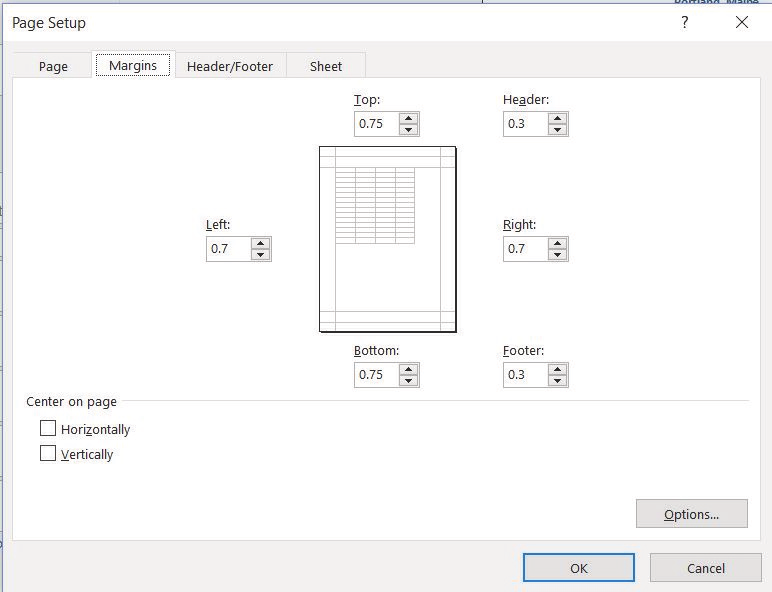
\includegraphics[width=\maxwidth{.95\linewidth}]{gfx/ch05_fig26}
	\caption{Page Setup}
	\label{05:fig26}
\end{figure}





2.   Click on the Margins tab.
3.   In the Center on page section, check the box for Horizontally.
4.   Click OK. The table should now be centered horizontally on the page.
5.   Next you need to add a footer with the workbook filename as well as the worksheet name.
6.   Open the Page Setup dialog box again (see Step 1 above).
7.   Click the Header/Footer tab then click the Custom Footer button.
8.   In the Left section: box type File:.
9.   Making sure to leave a space after the colon, click the Insert File Name button.
10.   In the Right section: box type Worksheet:.
11.   Making sure to leave a space after the colon, click the Insert Sheet Name button.
12.   The Footer dialog box should look like Figure 5.27. Click the OK button twice to return to Print
Preview. Confirm that the footer appears correctly, then exit Backstage View.



\begin{figure}[H]
	\centering
	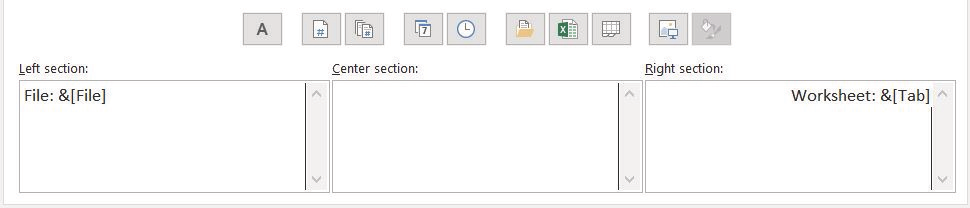
\includegraphics[width=\maxwidth{.95\linewidth}]{gfx/ch05_fig27}
	\caption{Custom Footer}
	\label{05:fig27}
\end{figure}





Inserting an Image to Enhance a Worksheet

Next you are going to add a small weather related graphic to the worksheet to enhance its appearance.
In Excel you can either insert an image file that you have saved or you can search for one online within
Excel. In this example, there is a graphic saved in the data files for this chapter that you will use.

1. Click the Insert tab on the ribbon.
2. Click the Pictures button from the Illustrations group. (This allows you to insert an image you
have saved. If you wanted to search for an image online, you would click the Online Pictures
button.) (See Figure 5.28.)


\begin{figure}[H]
	\centering
	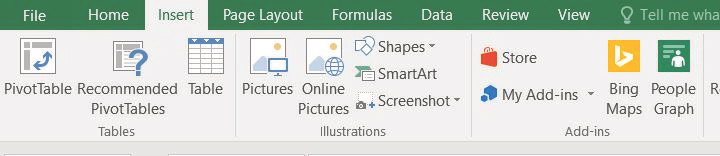
\includegraphics[width=\maxwidth{.95\linewidth}]{gfx/ch05_fig28}
	\caption{Insert Pictures}
	\label{05:fig28}
\end{figure}





3. Navigate to the location where your data files for Chapter 5 are located and double-click on the
Weather image file.

The image now appears on your worksheet, but not in the location you want. It is also slightly larger
than you would like. (See Figure 5.29.) You are going to move the image to cell E1, then resize it so it
does not cover up part of the table.


\begin{figure}[H]
	\centering
	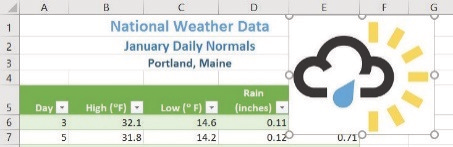
\includegraphics[width=\maxwidth{.95\linewidth}]{gfx/ch05_fig29}
	\caption{Inserted Image}
	\label{05:fig29}
\end{figure}





1. Place your pointer in the image so that the  (Note: ch05\_fig98 is here)   appears. Drag the image so that the top left corner
is in cell E1.
2. Using the resizing handle in the bottom right corner of the image, resize the image so that it
does not cover any of the table. Hint: drag diagonally to the left and up.
3. Check Print Preview again to make sure the worksheet with the image added looks good.
4. Exit Backstage View and save the Excel file.

\subsection{Previewing the Remaining Worksheets}

Before considering this workbook complete finished, you need to confirm that the remaining
worksheets are all printing appropriately.

1. Click the Portland OR worksheet and go to Print Preview. No changes need to be made to this
worksheet. Exit Backstage View.
2. Click the Weekly OR worksheet and go to Print Preview. Notice that the Slicer is printing on a
second page. To fix this, set the Page Scaling to Fit All Columns on One Page.

Notice that the last Slicer button (Saturday) is being cut off. This is because the Slicer height needs to
be adjusted.

1. Exit Backstage View.
2. Resize the Slicer so that all of the buttons display.
3. Return to Print Preview and confirm the worksheet, including the slicer, is printing
appropriately. Exit Backstage View.
4. Click the Subtotal OR worksheet and go to Print Preview.
5. Using the Page Setup dialog box, center this worksheet horizontally on the page.
6. Exit Backstage View.
7. Save the CH5 National Weather workbook.
8. Compare your work with the self-check answer key (found in the Course Files link) and then
submit the CH5 National Weather workbook as directed by your instructor.


Key Takeaways


• When working with Excel workbooks, the final step should always be to review the worksheets in Print
Preview to make sure they are printing appropriately.

• You can add images you have saved, or images you find online, to a worksheet to enhance its appearance. Be
sure to resize and move them appropriately so they do not detract from the data.



\section{Chapter Practice}




\subsection{Tables for a Tourism Company}

Download Data File: PR5 Data

\begin{figure}[H]
	\centering
	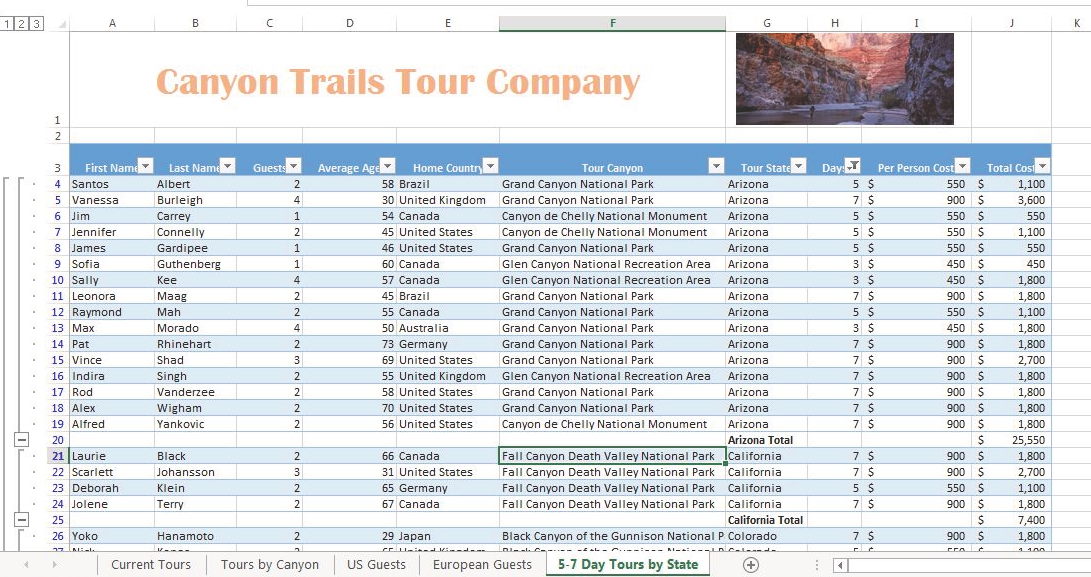
\includegraphics[width=\maxwidth{.95\linewidth}]{gfx/ch05_fig30}
	\caption{Chapter Practice Completed Exercise}
	\label{05:fig30}
\end{figure}






Travel and tour companies need to keep track of client data, as well as, travel/tour options and tour
guides. Keeping up-to-date, accurate records is essential to their bottom line. To run a tour company,
employees must be able to manipulate their data quickly and easily. This exercise illustrates how to use
the skills presented in this chapter to generate the data needed on a daily basis by a tourism company.
See Figure 5.30 above.

1. Open the data file PR5 Data and save the file to your computer as PR5 Canyon Trails.
2. In Column J, calculate Total Cost (number of Guests *Per Person Cost). Copy the formula down
the column.
3. Format Columns I and J with Currency and no decimal places.
4. Center all headings in Row 3.
5. Click in cell A3. Insert a table with headers for the range A3:J53.


6. Adjust column widths within the table so that all the headings are completely visible.
7. Rename Sheet 1 Current Tours. Sort this sheet alphabetically (A to Z) by Last Name.
8. Make a copy of the Current Tours sheet and rename it Tours by Canyon. Place the Tours by
Canyon sheet to the right of the Current Tours sheet. Sort this sheet by Tour Canyon (A to Z),
then Home Country (A to Z), and then Last Name (A to Z).
9. Make another copy of the Current Tours sheet and rename it US Guests. Place the US Guests
sheet to the right of the Tours by Canyon sheet. Filter this sheet so that only guests with a Home
Country of the United States show. Sort the filtered data alphabetically (A to Z) by Tour State.
Add a Total Row that sums the Guests and Total Cost columns.
10. Make another copy of the Current Tours sheet and rename it European Guests. Place the
European Guests sheet to the right of the US Guests sheet. Hide the Average Age column.
11. Insert a slicer in the European Guests sheet for Home Country. Move the top left corner of the
slicer to the top left-hand corner of cell K3. Change the width of the entire slicer to 1.65”.
12. Select both Germany and the United Kingdom on the slicer. Sort the filtered sheet by Home
Country (A to Z) and then Last Name (A to Z).
13. Make one more copy of the Current Tours sheet and rename it Tours by State. Place the Tours
by State sheet to the right of the European Guests sheet. Subtotal the sheet by State, summing
the Total Cost column.
14. Change the name of the Tours by State sheet to 5-7 Day Tours by State. Filter out 3 day tours in
the table.
15. On each worksheet, make the following print setup changes:

1. Add a footer with the worksheet name in the center.
2. Change to Landscape Orientation
3. Set the scaling to Fit All Columns on One Page

16. For any worksheets that print on more than one page, add Print Titles to repeat the first three
rows at the top of each page.
17. Save the PR5 Canyon Trails workbook.
18. Make sure your sheets are in the following order from left to right: Current Tours, Tours by
Canyon, US Guests, European Guests, and 5-7 Day Tours by State.
19. Compare your work with the self-check answer key (found in the Course Files link) and then
submit the PR5 Canyon Trails workbook as directed by your instructor.


\section{Scored Assessment}




\subsection{Tables for a Retail Company}

Download Data File: SC5 Data


\begin{figure}[H]
	\centering
	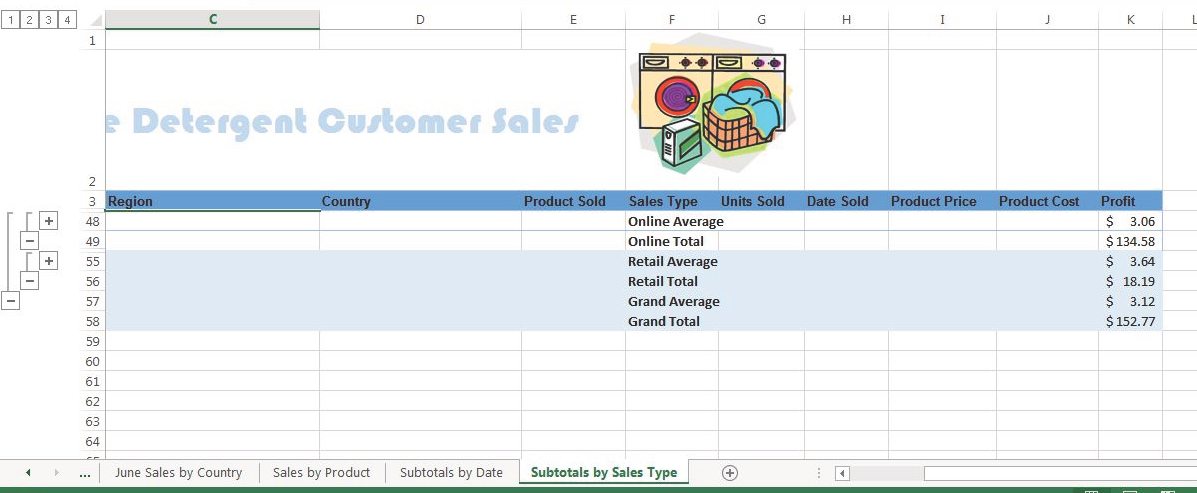
\includegraphics[width=\maxwidth{.95\linewidth}]{gfx/ch05_fig31}
	\caption{Scored Assessment Completed Exercise}
	\label{05:fig31}
\end{figure}



Retail companies with today’s online, as well as, in-store sales have a lot of data to keep track of!
Keeping track of sales, costs, and profits on a daily basis is essential to making the most of a business.
This exercise illustrates how to use the skills presented in this chapter to generate the data needed on
a daily basis by a retail company. See Figure 5.31 above.

1. Open the data file SC5 Data and save the file to your computer as SC5 Dynamite Customer
Sales.
2. Click on the Sales sheet. In I4 , enter a VLOOKUP function that will find the Product Price for
the Product in E4 in the table in the Product Table sheet and return it to I4. In your VLOOKUP
function, fill in the required parameters using Figure 5.32 below. Copy the VLOOKUP function
down column I.


\begin{figure}[H]
	\centering
	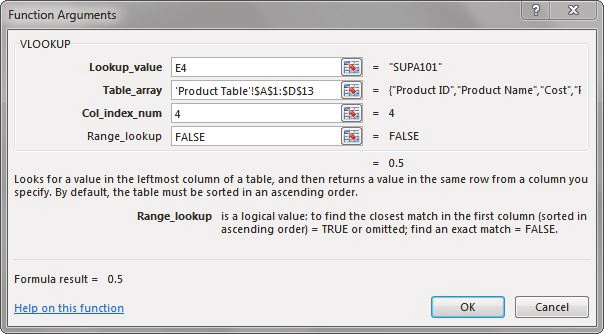
\includegraphics[width=\maxwidth{.95\linewidth}]{gfx/ch05_fig32}
	\caption{VLOOKUP window}
	\label{05:fig32}
\end{figure}






3. In J4 , enter a VLOOKUP function that will find the Product Cost for the Product in E4 in the
table in the Product Table sheet and return it to J4. This VLOOKUP function will be the same as
the %VLOOKUP function in I4 – EXCEPT THE COL_INDEX_NUM will be 3 instead of 4. Copy
the function down column J.
4. In K4, calculate Profit (Product Price – Product Cost). Copy this formula down column K.
5. Format columns I, J, and K as currency with two decimal places.
6. Click in cell A3. Insert a table with headers for the range A3:K52. BE CAREFUL HERE: Excel
will try to insert a table starting with A2. You want to make sure your range starts with A3 here.
7. Make a copy of the Sales sheet and rename it Online Sales by Date. Place this sheet to the right
of the Sales sheet. Filter out Retail in Sales Type, so that only Online Sales are displayed. Sort the
filtered data by Date Sold (oldest to newest).
8. Make a copy of the Sales sheet and rename it June Sales by Country. Place this new sheet to the
right of the Online Sales by Date sheet. Filter this sheet to only show June dates by using the
Date Filter Between. Sort this sheet alphabetically (A to Z) by Country and then alphabetically
by Name.
9. Make another copy of the Sales sheet and rename it Sales by Product. Place this new sheet to
the right of the June Sales by Country sheet. Hide the Region column.
10. Insert a slicer in the Sales by Product sheet for Product Sold. Move the top left corner of the
slicer to the top left-hand corner of cell M1. Resize the height of the entire slicer to 2.09”.
11. Select both DETA100 and DETA200 in the slicer. Sort the filtered sheet by Product Sold. Add a
Total Row that includes the overall average for the Product Price, Product Cost, and Profit
columns. Change the heading in A53 to Average.
12. Make a copy of the Sales sheet and rename it Subtotals by Date. Place this new sheet to the
right of the Sales by Product sheet. Subtotal the sheet by Date (Oldest to Newest), summing the
Profit column. Click the 2 Outline button to show just the subtotals by date and the grand total.


13. Make one final copy of the Sales sheet and rename it Subtotals by Type. Place this new sheet to
the right of the Subtotals by Date sheet. Subtotal the sheet by Sales Type, summing the Profit
column.
14. Add a 2nd subtotal to the Subtotals by Type sheet that subtotals by Type and averages the Profit
column. (Hint: uncheck Replace Current Subtotals in the Subtotal dialog box.) Notice that 4
Outline buttons appear with the 2nd subtotal. Figure out which Outline button to click to
display both subtotals for Online and Retail and two Grand Totals.
15. For each worksheet, add a footer with the worksheet name in the center.
16. Preview each worksheet in Print Preview and make any necessary changes for professional
printing. (Hint: Orientation, page scaling, and print titles might need to be used)
17. Double-check that your sheets are in the following order from left to right: Sales, Online Sales
by Date, June Sales by Country, Sales by Product, Subtotals by Date, Subtotals by Sales Type,
and Product Table.
18. Save the SC5 Dynamite Customer Sales workbook.
19. Submit the SC5 Dynamite Customer Sales workbook as directed by your instructor.

